\chapter{Implementation}
\label{chap:Implementation}
In this chapter we explain the infrastructure that performs all the necessary steps to produce an efficient feedback. A general overview is given and for each section, we describe in particular the tools as well as the way we manipulated the data in order to obtain the information useful for the user. The chapter is divided in two parts: the first part focuses on the back-end and the services we used to extract the features we described in \ref{chap:Speech Recognition}. The second part describe the front-end, that is, the \textit{Android}\footnote{\url{https://www.android.com}} application (called \textbf{PARLA}\footnote{\url{https://github.com/davideberdin/PARLA}}) with a particular focus on the feedback page and the general usage.

\section{General architecture}
\label{sec:general_architecture}

In \ref{fig:general_architecture} is shown the general architecture of the infrastructure.
The flow displays only the \textit{pronunciation testing} phase:

\begin{itemize}
	\item[1)] User says the sentence using the internal microphone of the smartphone (or through the headset)
	\item[2)] The application sends the audio file to the \textit{Speech Recognition service}
	\item[3)] The result of step 2 is sent to the \textit{Gaussian Mixture Model service}
	\item[4)] The result of step 3 is sent back to the application where a \textit{Feedback page} is displayed
	\item[5)] A short explanation for each chart is given to the user
	\item[6)] Back to step 1
\end{itemize}

\noindent The flow described above is the main feature of the whole project. Although, the application supplies other two important functionalities that are described more in detail in \ref{sec:android_app}. The first one is related to \textbf{critical listening} where the user is able to listen to the \textit{Native pronunciation} as well as to its one. This feature have a big impact on improving the pronunciation because it pushes the user to understand the differences as well as to emulate the way native speakers pronounce a specific sequence of words. The second feature regards the \textbf{history} (or progress). This page shows the trend of the user based on all the pronunciation he/she made during the usage of PARLA. The purpose of the history page is to help the user to see the progresses and to get an idea of how to improve the pronunciation. \\

\begin{figure}[!ht]
	\centering
	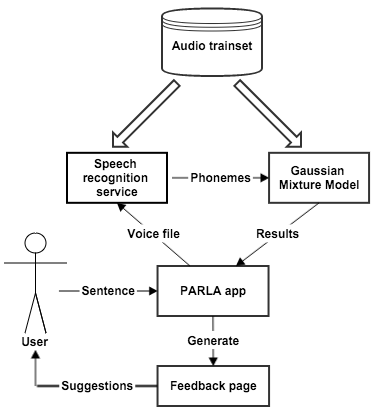
\includegraphics[scale=0.6]{Figures/general_architecture.png}
	\caption{General architecture of the infrastructure}
	\label{fig:general_architecture}
\end{figure}

\subsubsection{Implementation procedure}
\label{ssec:procedure}

Several step were made before to reach the architecture depicted in \ref{fig:general_architecture}. Generally speaking, we divided the implementation in two main categories: the first is composed by the \textit{data collection and training} phase whereas the second is formed by the \textit{mobile application} and \textit{server communication}. \\

\noindent The very first step was to collect the data from native speakers and apply some pre-processing techniques in such way that we were able to obtain only the information we needed to train the two services we had on the server.After the data collection, we trained both the models with the information we extracted in the previous step. The detailed procedures are described in \ref{ssec:training_sr_model} and \ref{ssec:training_gmm}. \\
\noindent When the training phase was completed, we set up the services and used \textit{REST} calls to communicate with the mobile application. These two parts were developed at the same time and are described in detail in \ref{sec:android_app}.


\section{Data collection}
\label{sec:data_collection}

The data collection step is a crucial phase of the entire project. The reason for such importance is that the audio record has to be clear, clean and as natural as possible. In fact, the people who participate to this phase were asked to pronounce the sentences as they would say in a day-by-day conversation. \\

\noindent We recorded 8 people divided in 4 males and 4 females at the University of Rochester using \textit{Audacity}\footnote{\url{http://audacityteam.org}}. Each person had to pronounce 10 sentences (see \ref{table:sentences}) and each sentence was pronounced 10 times. \\
\noindent The sentences were chosen in order to cover the most used English sounds and based on the frequencies of everyday usage\footnote{\url{http://www.learn-english-today.com/idioms/idioms_proverbs.html}}.

\begin{table}[!ht]
	\centering
	\begin{tabular}{|c|c|}
		\hline
		\multicolumn{2}{|c|}{Sentences}      \\ \hline
		A piece of cake  & Fair and square   \\ \hline
		Blow a fuse      & Get cold feet     \\ \hline
		Catch some zs    & Mellow out        \\ \hline
		Down to the wire & Pulling your leg  \\ \hline
		Eager beaver     & Thinking out loud \\ \hline
	\end{tabular}
	\caption{Idioms used for testing the pronunciation}
	\label{table:sentences}
\end{table}

\noindent The total file we gathered were 800 and the average length of each file is \textbf{1s}. In total, we were able to gather 14 minutes of recorded audio. This amount of time was sufficient for training the speech recognition model and the GMM. In reality, for the speech recognition service, we initially trained the model with a bigger dataset and then we added the one with the sentences (details in \ref{fig:sphinx_service}). The reason is that the tool we used for the speech recognition, requires a large dataset\footnote{\url{http://cmusphinx.sourceforge.net/wiki/tutorialam}}.

\subsection{Data pre-processing}
\label{ssec:pre_processing}

The data pre-processing step is one of the most important procedure of the whole project. In fact, extracting the right information is crucial for both training the models and those voice-features that should be showed to the user. \\

\noindent The process starts by using the tool called \textbf{PRAAT}\footnote{http://www.fon.hum.uva.nl/praat/}. This tool is used for \textit{analysis of speech in phonetics} as well as for \textit{speech synthesis} and\textit{articulatory synthesis} \cite{boersma2001praat}. With PRAAT, we were able to analyze the audio files we collected in the very beginning of the project and extracting formants and stress. In \ref{sub:formants} and \ref{sec:stress} we detailed explained the meaning of these parameters. \\
From here, we generated a set of \textit{CSV} files where we saved the values of the formants and the stress for each audio file. These file are then used as input for a tool called \textbf{FAVE-Align}\cite{yuan2008speaker}. \\

\noindent FAVE-Align is a tool used for \textit{force alignment}. This process is used to determine where a particular word occurs in an audio frame \cite{forced_alignment_def}. In other words, FAVE-Align takes a text transcription and produce a PRAAT TextGrid file where it shows when those words start and end in the related audio file. In \ref{fig:fave-align_result}, there is an example of this procedure. The tool performs different phases in order to align audio and text.\\

\noindent The first step is to sample the audio file and apply the Fourier Transformation because there is the need to move from the \textit{time domain} to \textit{frequencies domain}. From here, the tool extract the \textit{spectrum} and apply the Inverse Fourier Transformation on it to obtain the so called \textbf{Cepstrum}. The \textit{cepstrum} is the representation in a small-window frame of the spectrum. Although, the amount of information extracted from the cepstrum are too high, and for this reason, the tool uses \textit{Perceptual Linear Prediction coefficients} to retrieve the necessary data to perform the alignment decision. These coefficients are used for feature extraction. The detailed process can be found at \cite{hermansky1990perceptual}. \\
The last part of this process is the decision making part and this is done by a \textit{Hidden Markov Model}. \\

\begin{figure}[!ht]
	\centering
	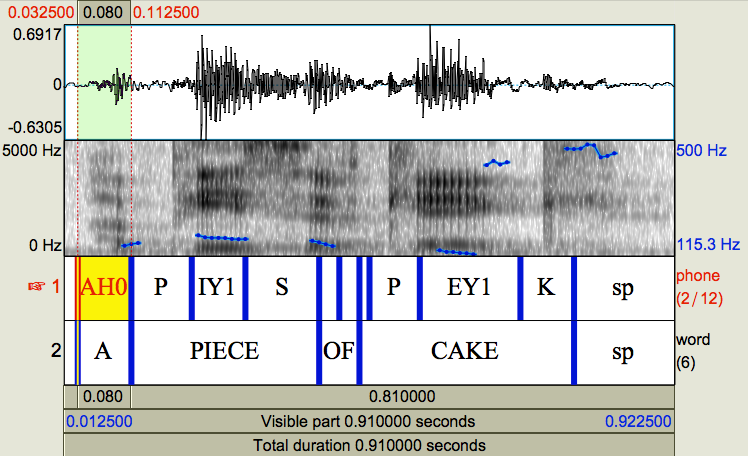
\includegraphics[scale=0.4]{Figures/fave_align.png}
	\caption{Result from FAVE-Align tool opened in PRAAT}
	\label{fig:fave-align_result}
\end{figure}

\noindent The outcome of the previous step is used as input for the tool called \textbf{FAVE-Extract}. This tool helps to automates the vowel formant analysis. The process is dived in two main steps: the first is finding the \textit{Measurement Points} and the second is the \textit{Remeasurement}. \\

\noindent In \cite{rosenfelder2011fave} is explained that for most vowels it is possible to find the measurement point by listening 1/3 of the total duration. This point is necessary for determining the identity of the vowel, that is, the name of the vowel itself. For more complex vowels, a different approach is done, that is, the point is halfway between the F1 (main formant) maximum value and the beginning of the segment. In addition, the LPC analysis is performed on both beginning and end of the vowel in order to pad the vowel's window. This \emph{ensure a formant track through the full vowel's duration}\cite{harrison2004variability}. The result of this step is a set of candidates. This set is composed by the potential formants estimated from the likelihood of the \textbf{ANAE} distribution. The \textit{Atlas of North American English} (ANAE) is the set of phonology formants values depending on the English regional area. The winner formant is determined by the Posterior probability. This step does not take in consideration the provenience of the speaker. \\

\noindent The second part of the formants extraction tool is to remeasure the parameters by adjusting the ANAE distribution based on the regional area of the speaker. In this way, the formant value will be more accurate. An example of result from FAVE-Extract is shown in \ref{fig:fave-extract_example}.

\begin{figure}[!ht]
	\centering
	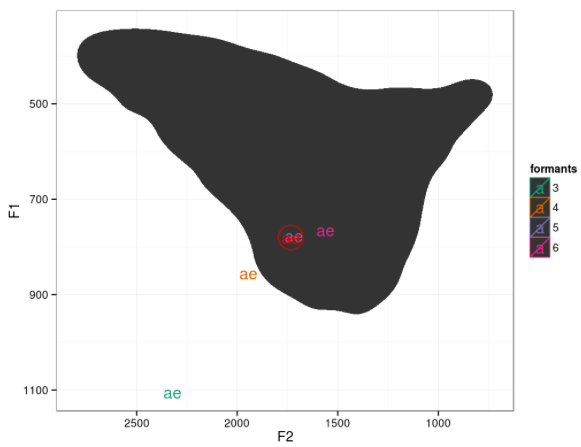
\includegraphics[scale=0.5]{Figures/fave-extract_example.png}
	\caption{Result from FAVE-Extract}
	\label{fig:fave-extract_example}
\end{figure}

\noindent The result of the data pre-processing is a set of information composed by the average value of F1, F2 and F3 formants with their respectively vowels text representation. The formants values will be then used to train both the speech recognition model and the Gaussian Mixture Model.

\section{Server}
\label{sec:server}

The back-end system is divided in two different services: the first one handles the speech recognition converting the user's voice into a set of phonemes, whereas the second service is in charged of all the other operations a user can do, such as login/logout, history data, vowels prediction system, usage collection, etc.. This section explains more in detail how we extract the information from the audio files and how we manipulate those before to give the feedback to the user.

\subsection{Speech Recognition service}
\label{ssec:training_sr_model}

The first service in order of usage within the whole system, is the speech recognition one. This has been made possible by using the well-known \textbf{CMU-Sphinx} software by Carnegie Mellon University \cite{walker2004sphinx}. The framework is written in Java and it is completely open-source. The system has been deployed on a \textit{Tomcat}\footnote{https://tomcat.apache.org} service as Java Servlet to serve the requests from the Android application. \\

\begin{figure}[!ht]
	\centering
	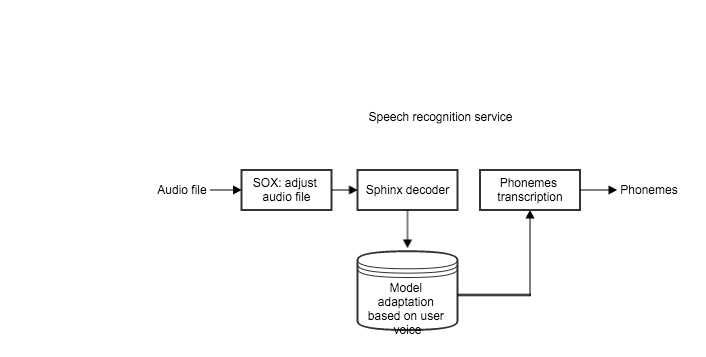
\includegraphics[scale=0.6]{Figures/sphinx_service.png}
	\caption{Architecture of the Speech recognition service}
	\label{fig:sphinx_service}
\end{figure}

\noindent The first phase consisted in training the audio model with two different language models. The first (and bigger) is the \textit{Generic U.S. English model} whereas the second is composed by the data audio-files we collected from the native speakers. The first dataset is directly provided by the tool and already embedded in the decoder. This means that, the system has been already trained with a generic model so that new developers do not have to collect data to train the model. We are a special case because we wanted to focus the attention on only 10 specific sentences and in order to specialize the language model, we had to add specific files. This phase took several hours of work because the amount of data we used was very large. \\

\noindent Once the model has been trained, we are then ready to adjust the parameters based on the voice of the user. For this task, CMU-Sphinx provides a particular method that permits the model to be adapted based on pitch and speed-of-speech of the user. To do so, we had to build the system in such a way that for each user, a specific file with the voice's parameters was created. In this way, CMU-Sphix would retrieve improve the recognition every time a user feeds the system with audio files. \\

\noindent At this point the system is trained and ready to recognize. When the service receives an audio file, the first step before proceeding to CMU-Sphinx is to change some properties of the audio file itself. In fact, the Sphinx decoder has the best performance only when the audio files are in \textit{mono-channel} and have a sampling frequency of \textit{16Khz}\footnote{http://cmusphinx.sourceforge.net/wiki/faq}. The library we used to record the user in PARLA, is sampled in \textit{stereo-channels} and \textit{11Khz}. For this reason, we used a special tool called \textbf{SOX}\footnote{http://sox.sourceforge.net} that helped us to change the properties of the audio file according to the required ones. \\

\noindent Once the file has been manipulated, we retrieve the voice's parameters file of the user and start the recognition part. CMU-Sphinx goes through several internal procedures (general details in \ref{chap:Speech Recognition}) and during this process it adapts the model based on the user's voice. On the end of the whole process, a string containing the phonemes of the pronounced sentence is given back as result. An example is given in \ref{fig:result_sphinx}. The red box indicates the result we took in consideration.

\begin{figure}[!ht]
	\centering
	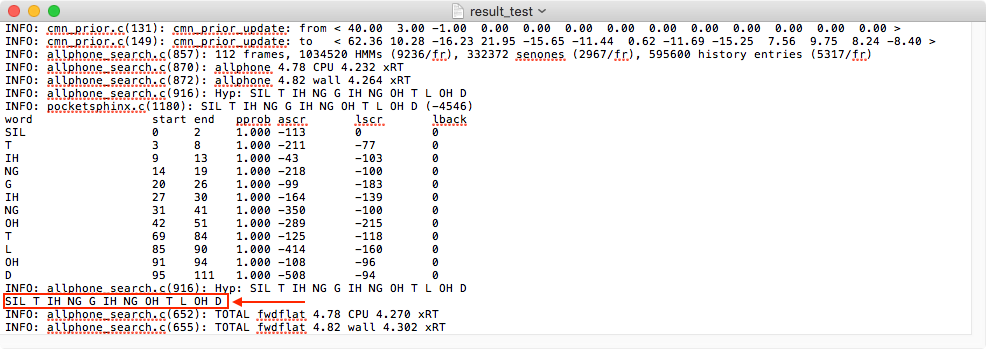
\includegraphics[scale=0.5]{Figures/result_sphinx.png}
	\caption{Example of phonemes recognition using CMU-Sphinx for the sentence \textit{Thinking out loud}. The phoneme \textbf{SIL} stands for \textit{Silence}}
	\label{fig:result_sphinx}
\end{figure}

\subsection{Voice analysis system}
\label{ssec:training_gmm}

The second service we built, handles the analysis of the audio file in order to give feedback to the user. This process is long because it involves several steps and sometime the user had to wait up to 40 seconds before to get the results. In \ref{fig:gmm_service} is depicted the macro-view of the service's architecture. \\
\noindent The system was written in Python using Django\footnote{https://www.djangoproject.com} as web-framework. The choice was made based on the availability of machine learning libraries and the language tools (FAVE-extract and FAVE-align). In fact, we used \textit{scikit-learn}\footnote{http://scikit-learn.org/stable/}, a well-known python library for data-analysis, data mining and machine learning. \\

\begin{figure}[!ht]
	\centering
	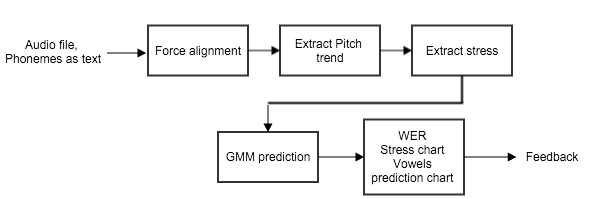
\includegraphics[scale=0.6]{Figures/gmm_service.png}
	\caption{Architecture of the Voice analysis service}
	\label{fig:gmm_service}
\end{figure}

\subsubsection{Training GMM}

\noindent As for the speech recognition service, we had to train the Gaussian Mixture Model with the audio features of the native speakers. As we explained in \ref{ssec:pre_processing}, we used formants F1, F2 and F3 as training dataset for this model. In fact, the first three formants are sufficient for recognizing the phoneme that has been pronounced. According to \cite{prica2010recognition}, the first two formants are not sufficient for discriminating the \textit{"value"} of the phoneme due to a big overlapping in their spectrum. Using the third formants, we can catch those frequencies that can act as decision makers. \\

\noindent Scikit-learn provides a GMM out of the box. Although, the number of parameters available make it hard to properly set the model. For this reason, we used a method called \textbf{Bayesian information criterion} (BIC) to find the optimal solution for our purpose. \\

\noindent BIC is a model selection method that gives a score on an estimated model performance based on a testing dataset. Lower the score, better is the model.\\
\noindent In \ref{eq:bic} is defined the formula used for calculating the score, where $T$ is the size of the training set, $\ln{\hat L}$ is the maximum likelihood value of the given model (details in \ref{sec:mle}) whereas $k$ is the number of \textit{free} parameters that can be estimated. \\
\noindent When the BIC method is attempted, it tries to avoid the risk of \textit{overfitting} the model by injecting a \textit{penalty term} of $k \cdot \ln(T)$ that augment proportionally with the number of parameters \cite{bic_info}. This term also helps to avoid unnecessary parameters and keep the model as simple as possible. In \ref{fig:bic1} and \ref{fig:bic2} are shown the BIC evaluation.

\begin{equation}
\label{eq:bic}
	 BIC = -2 \cdot \ln{\hat L} + k \cdot \ln(T)
\end{equation}

\noindent Given the results of the evaluation, we selected the model's parameters with the lowest BIC score. In \ref{lst:gmm} is shown the code we used to create the classifier after having run the BIC evaluation.

\begin{lstlisting}[caption={Parameters of GMM classifier},label={lst:gmm}, style=BashInputStyle]
gmm_classifier = mixture.GMM(n_components=12, covariance_type='full',
			     init_params='wmc', min_covar=0.001, n_init=1,
			     n_iter=100, params='wmc', random_state=None,
	                     thresh=None, tol=0.001)
\end{lstlisting}

\clearpage

\noindent The next list of parameters are those that have been automatically selected by the evaluation whereas the others are set by default:

\begin{itemize}
	\item \textit{Number of components} decided based on the total amount of possible phonemes (in our case, 12)
	\item \textit{Covariance type} set to \textbf{full} as indicated by BIC
	\item \textit{Initial parameters} updated by \textbf{weight}(w), \textbf{means}(m) and \textbf{covariance}(c)
	\item \textit{Tol} is the convergence threshold. The Expected Maximization breaks when the average gain log-likelihood is below \textbf{0.001}
\end{itemize}

\noindent After the training part, we tested the classifier with a testing set composed by the first 3 Formants that we extracted using PRAAT from 5 audio files provided by the same person. Both \textit{Training accuracy} and \textit{Testing accuracy} were calculated using the function \textbf{numpy.mean()} where the average is computed along the axes that has been specified.

\begin{lstlisting}[caption={Code for accuracy estimation of training and testing set},label={lst:accuracy}, style=BashInputStyle]
train_accuracy = numpy.mean(y_train_predicted == y_train) * 100
test_accuracy = numpy.mean(y_test_predicted == y_test) * 100
\end{lstlisting}

\noindent In \ref{table:accuracy} are shown the results after the training of Gaussian Mixture Model. The accuracy values can be improved by increasing the amount of training data.

\begin{table}[!ht]
	\centering
	\caption{Testing results after the training}
	\label{table:accuracy}
	\begin{tabular}{|l|c|c|}
		\hline
		\multicolumn{1}{|c|}{\textbf{Sentence}} & \textbf{Training Accuracy}       & \textbf{Testing Accuracy}        \\ \hline
		A piece of cake                         & 								   &
		\\ \cline{1-1}
		Blow a fuse                             &                                  &                                  \\ \cline{1-1}
		Thinking out loud                       &  \textbf{82.5\%}                 & \textbf{90.7\%}
		\\ \cline{1-1}
		Mellow out                              &                                  &                                  \\ \cline{1-1}
		Eager beaver                            &                                  &                                  \\ \hline
	\end{tabular}
\end{table}

\subsubsection{Pitch, stress and Word Error Rate}
\noindent After the training phase, we built three other components that deal directly with the feedback the user will receive. In fact, we used PRAAT to extract the \textit{Pitch contour} in order to show the user, the way his/her voice changes compared to a native speaker. In \ref{fig:pitch_native} is shown an example of contour that we used as feedback for the user. In fact, it is possible to notice that both the natives have a similar way of saying the same sentence. This is a key point because the non-native will compare the way he/she will pronounce the sentence and understand the eventual differences. \\

\begin{figure}[!ht]
	\centering
	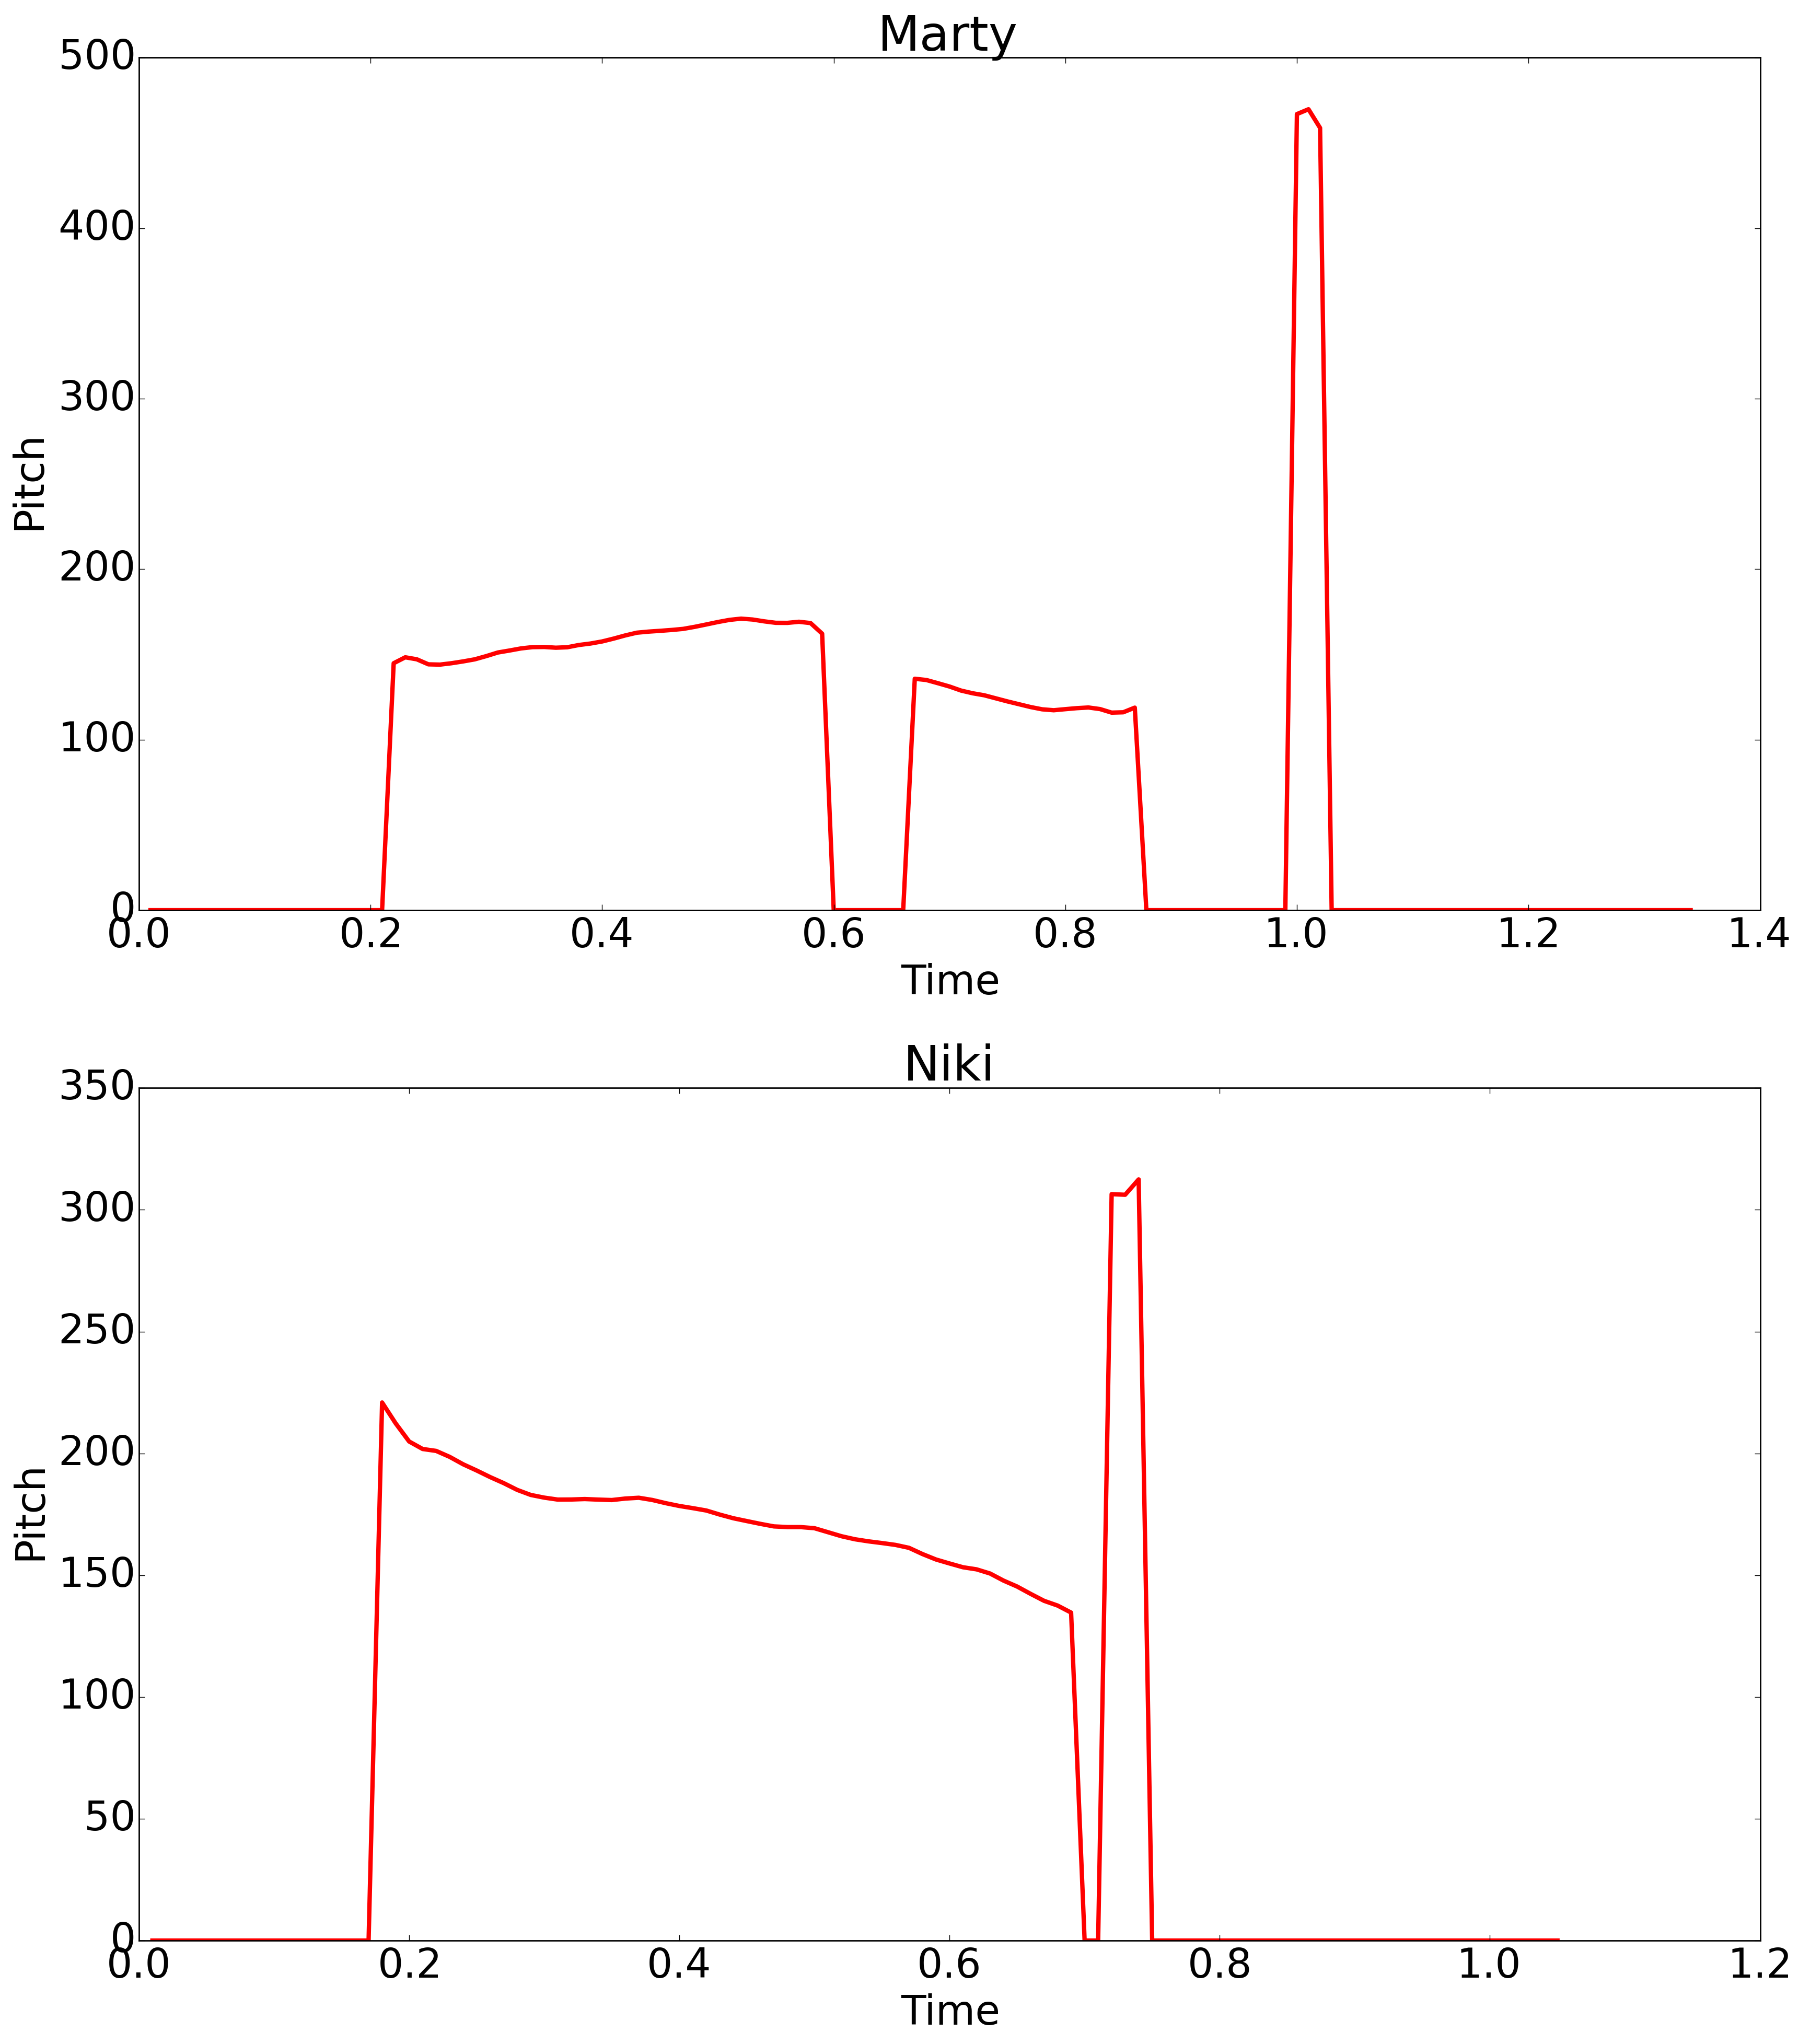
\includegraphics[scale=0.15]{Figures/pitch_native.png}
	\caption{Example of pitch contour provided by two native speakers for the sentence \textit{Mellow out}}
	\label{fig:pitch_native}
\end{figure}

\noindent Stress is extracted in a different way. Instead of using PRAAT, we decided to use \textit{FAVE-extract} because it provides a feature that retrieve the stress position(s) in the sentence. Moreover, it offers the opportunity to know on which phoneme the stress occurs. Given that, to the user it will be presented the phoneme representation of the pronounced sentence provided by the speech recognition service as well as in which phonemes the stress is emphasized. \\

\noindent Last piece of the system is to calculate the difference between the pronunciation of the native and the user, from the phoneme point of view. For this purpose, we decided to use a well-known evaluation metric system called \textbf{Word Error Rate} (WER). \\

\noindent WER is a common evaluation metric system to check the accuracy of a speech recognition's system. The main idea is to calculate the distance between the \textbf{hypothesis} and \textbf{reference}. The first is the result produced by the system whereas the second is the expected text. The distance is measured using the \textit{Levenshtein} algorithm, where it is calculated the minimum number of edits that it is needed to change one single character to another. Likewise, WER calculates the minimum amount of operations that has to be done for moving from the reference to the hypothesis. \\ \\ \\ \\

\noindent The possible edits are:

\begin{itemize}
	\item \textit{Insertion}: a word was added to the hypothesis
	\item \textit{Substitution}: an aligned word from the hypothesis has been substituted in the reference
	\item \textit{Deletion}: a word has been deleted in the reference
\end{itemize}

\noindent The calculations are done by putting each edit on a Levenshtein distance's table and then \textit{backtrace} in it through the shortest path to the origin $(0, 0)$ \cite{WER}. Each step during the backtrace is counted. After this, WER uses the formula in \ref{eq:wer} to calculate the \textit{error rate}.

\begin{equation}
\label{eq:wer}
	WER = \frac{S + D + I}{N}
\end{equation}

\noindent where S is the substitutions, D the deletions, I the insertions and N are the words in the reference text.


%%%%%%%%%%%%%%%%%%%%%%%%%%%%%%%%%%%%%%%%%%%%%%%%%%%%%%%%%%%%%%%%%%%%%%%%%%%%%%%%
%%%%%							ANDROID PART							   %%%%%
%%%%%%%%%%%%%%%%%%%%%%%%%%%%%%%%%%%%%%%%%%%%%%%%%%%%%%%%%%%%%%%%%%%%%%%%%%%%%%%%


\section{Android application}
\label{sec:android_app}

The choice of using the Android OS for developing the mobile application was in somehow forced by the fact that the other mobile OS do not allow installing application outside their respectively stores. In this way we could freely distribute the application and be more flexible regarding the implementation. \\
\noindent We used \textit{Android Studio}\footnote{http://developer.android.com/tools/studio/index.html} as IDE and the \textit{API level 21} where the minimum  Android version required is 5.0.

\subsection{Layouts}
\label{ssec:layouts}
The application is composed of four main layouts: \textit{pronunciation page}, \textit{feedback page}, \textit{history page} and \textit{critical listening page}. Among these, the \textbf{feedback page} is the most important one since it provides the differences with the native pronunciation. \\

\noindent The \textbf{pronunciation page} is depicted in \ref{fig:pronunciation_page} and it is possible to notice that the user has access to a multitude of options, such as: listening to the native speaker, change word, see the \textit{IPA} phonetics and, of course, test his/her pronunciation. \\

\noindent The \textbf{critical listening} section has been created to help the user to understand the differences between what he/she said and the native, based only on the audio. The page is split in two parts: on the left side there are all the native pronunciations whereas on the right there are all the non-native ones. For each sentence then it is possible to either \textit{test the pronunciation} or \textit{se the history}. The first choice redirects the user to the Main page whereas the second will show the eventual progress for that particular sentence. \\

\begin{figure}[!ht]
	\centering
	\begin{minipage}{.5\textwidth}
		\centering
		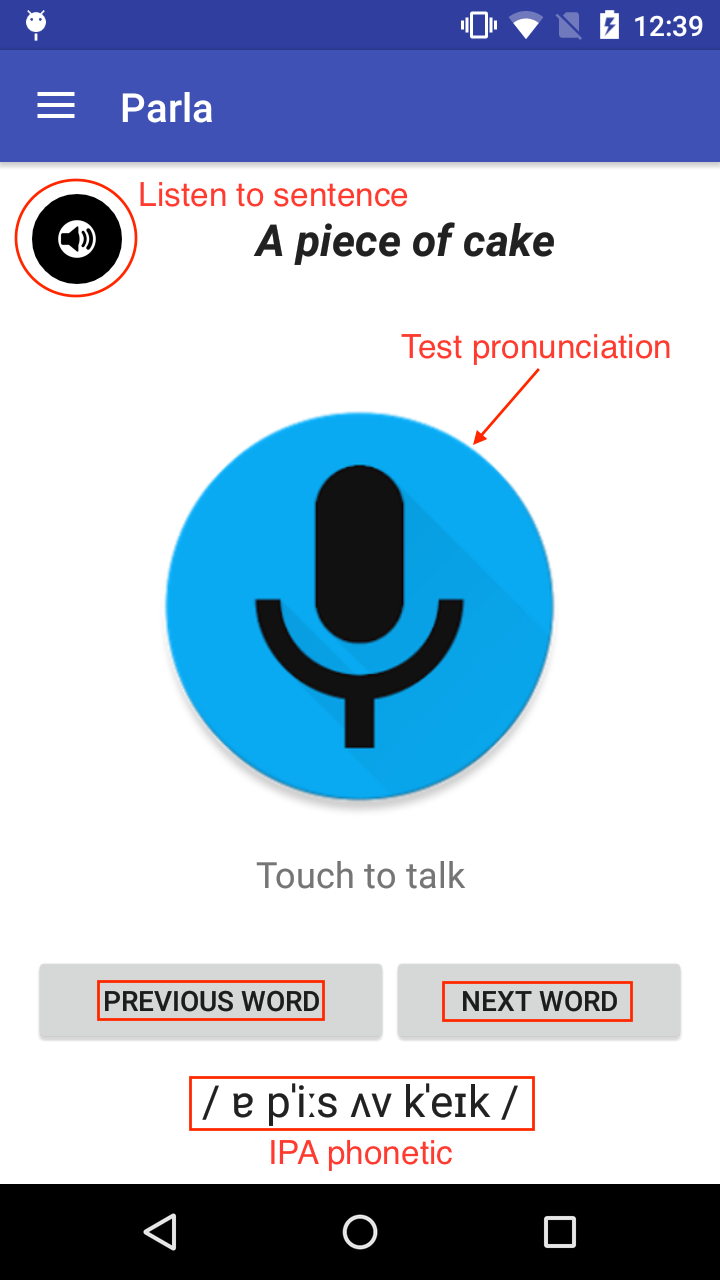
\includegraphics[scale=0.18]{Figures/screenshots/main.png}
		\caption{Pronunciation (or Main) page of PARLA}
		\label{fig:pronunciation_page}
	\end{minipage}%
	\begin{minipage}{.5\textwidth}
		\centering
		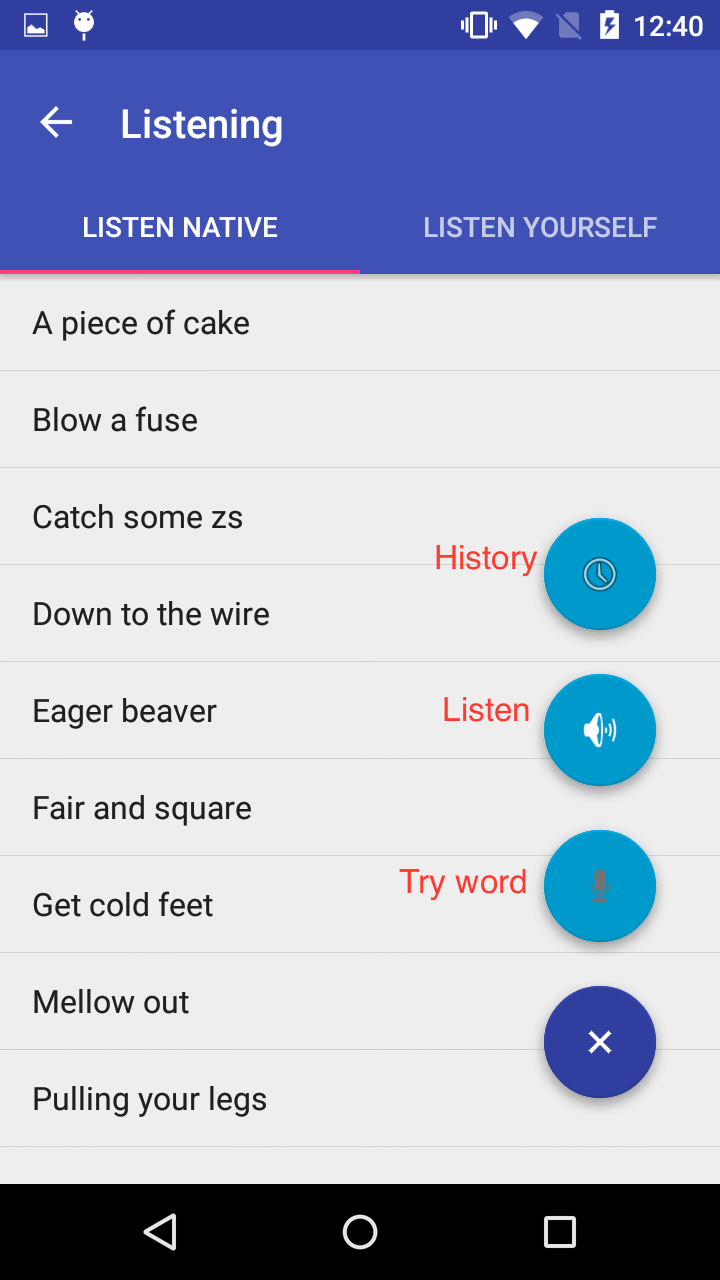
\includegraphics[scale=0.18]{Figures/screenshots/listening.png}
		\caption{Listening page}
		\label{fig:listening_page}
	\end{minipage}
\end{figure}

\noindent The \textbf{history page} provides a simple visualization of the user's progress. In \ref{fig:history_page} it is possible to notice that the page is split in two parts: the top part shows the vowels pronunciation of each time the user tested the pronunciation whereas the bottom part shows how \textit{close} the articulation of that specific vowel was to the native. \\

\noindent These layouts have been designed to provide the necessary information prior testing the pronunciation with the only exception of the history page. As said in \ref{ch:introduction}, \textit{listening} and \textit{phonetics} help the student to improve the quality of the pronunciation as well as the correctness. Keeping these statements in mind, we designed the pages in order to achieve the maximum effect. \\

\noindent During the development of the User Interface, we conducted a simple study where we asked a group of 4 people to interact with the sketches of the initial UI. The process was straightforward because we initially explained the purpose of this application and then what we wanted to achieve. The study was based on a sequence of questions aimed to improve the usability - here are the asked topics:

\begin{itemize}
	\item Navigation among pages
	\item Modifications in the main page
	\item Modifications in the critical listening page
	\item Modifications in the history page
	\item Modifications in the feedback page
	\item Add/Remove features
\end{itemize}

\noindent Based on the answers we changed the layouts accordingly.

\begin{figure}[!ht]
	\centering
	\begin{minipage}{.5\textwidth}
		\centering
		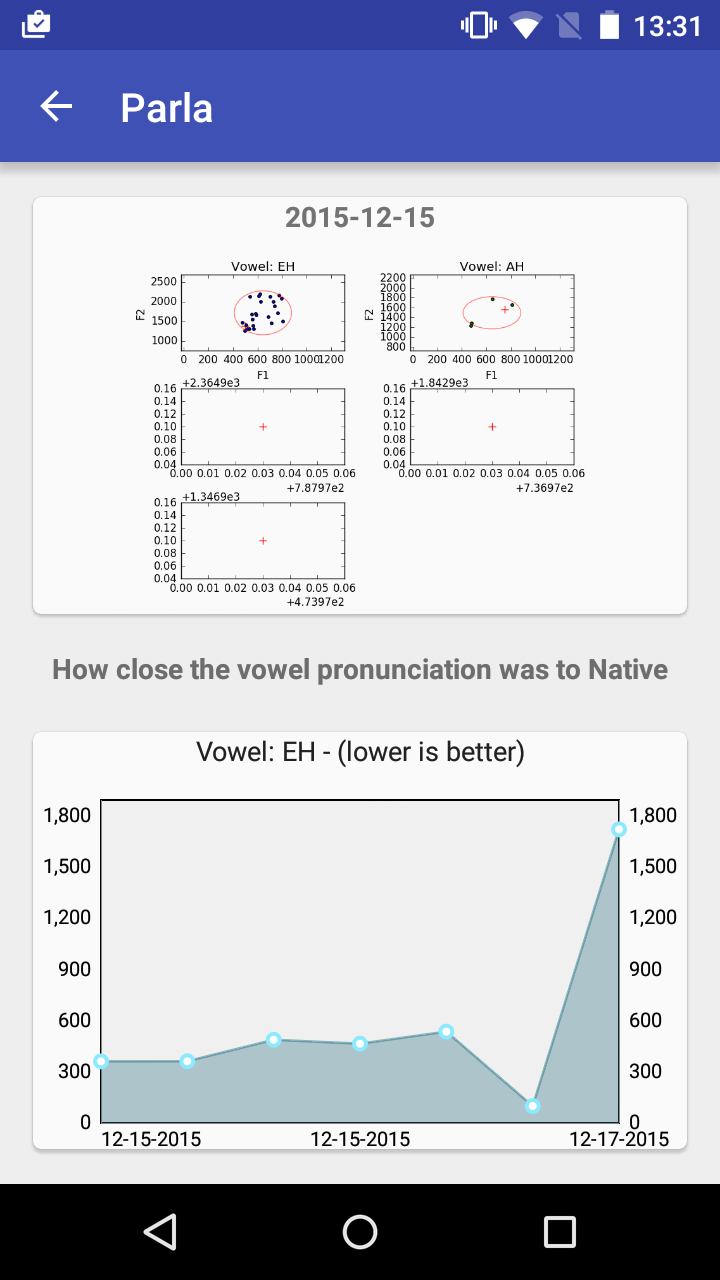
\includegraphics[scale=0.18]{Figures/screenshots/history2.png}
		\caption{Example of History page}
		\label{fig:history2_page}
	\end{minipage}%
	\begin{minipage}{.5\textwidth}
		\centering
		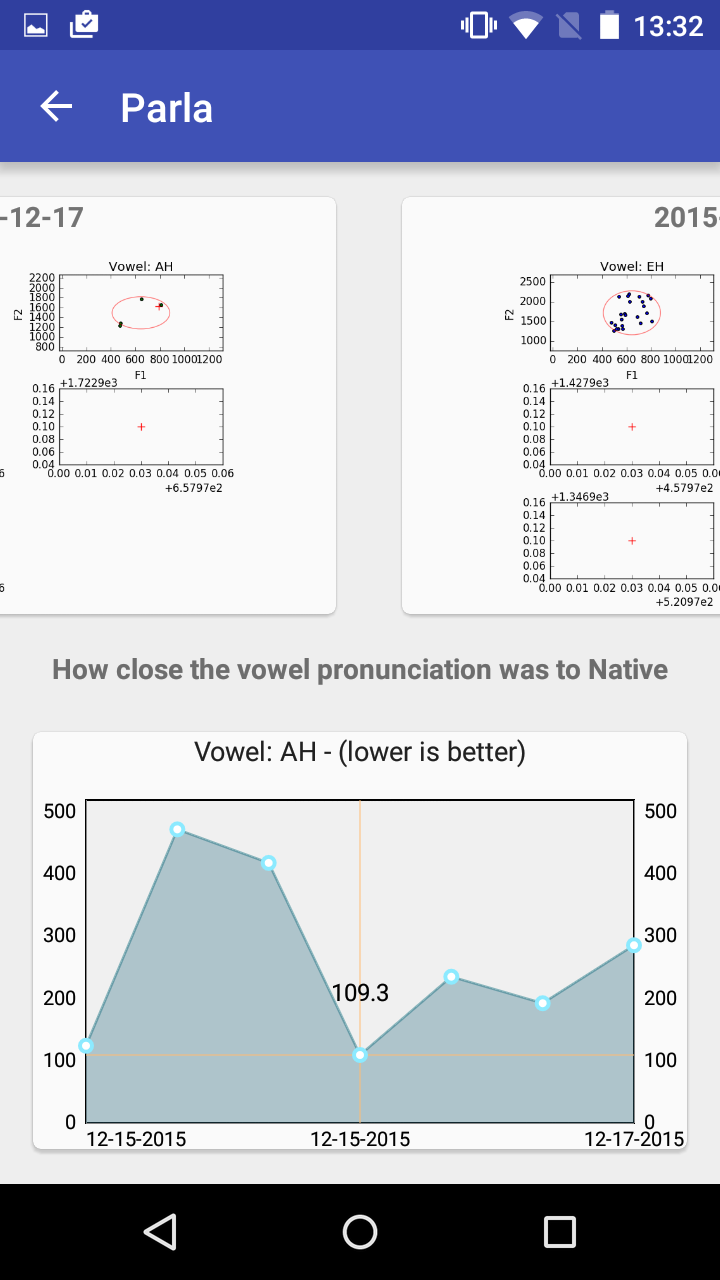
\includegraphics[scale=0.18]{Figures/screenshots/history.png}
		\caption{History page with interaction}
		\label{fig:history_page}
	\end{minipage}
\end{figure}

\subsection{Feedback layout}
\label{ssec:feedback_layout}
We reserved an entire section dedicated to the \textbf{feedback page} because this the core of the whole project. This page has been designed to provide as many information as possible giving the minimum explanation regarding the differences. Basically, we focused our attention in creating charts and the phonetics representations in order to give feedback. This page combine all the information from both the speech recognition system and the voice analysis service. \\

\noindent The page is divided in three main parts. The first part is represented by the phoneme representation and the WER located at the very top of the page. The button on top left provides the meaning of the sentence as well as a typical usage in a context.\\
\noindent For each sentence we show the comparison between the native and the user. In fact, as \ref{fig:error_rate_page} and \ref{fig:error_rate2_page} show, the user immediately can understand those differences if any. The syllables highlighted in red represent the \textbf{stress} of that particular sentence. In addition, the \textit{word error rate} shows how different was the user's pronunciation from the native speaker. The second picture shows that the user mispronounced the word \textbf{to}, that is why \textit{WER} is $10\%$. The stress is correct in both cases otherwise it would be highlighted. \\

\noindent The second part is represented by the chart in which the \textit{stress trend} is depicted. Here we provide a graphical representation of how the sentence should be emphasized. As for the first part, we show the difference between the native and the user. Although, the two trends will \textbf{never} be the same because the process of extracting this information involves the \textit{voice pitch} of a person. Basically, what the user should pay attention to, is the \textit{shape} of those lines. If the trends are similar, then it means that the stress is in the right position during the pronunciation. In \ref{fig:pitch_page} for example, it is shown a very bad pronunciation. In fact, WER is $75\%$ and the stress trend does not look like the native's one. The picture clearly shows the impact on a user when making mistakes in the pronunciation. \\

\noindent The last part of this page is represented by the \textit{vowels prediction} chart. Here we show the various pronunciation formants values of the vowels involved in a particular sentence. These values are extracted from the GMM in the voice analysis service. In \ref{fig:vowels_page} it is possible to notice how the vowels formants are well defined and clustered together. The circles represent the range of formants values in which that determined vowel should be pronounced. The \textit{red crosses} are the user's formants prediction. The feedback information here is that the user should understand that if the red cross is not within the circle and close to the group of green dots, then he/she should change the pronunciation. To learn this there are two ways: using the critical listening or looking at the numbers in the chart. The first method is simpler and more effective whereas the second option is for those that have a prior knowledge in linguistic. \\

\begin{figure}[!ht]
	\centering
	\begin{minipage}{.5\textwidth}
		\centering
		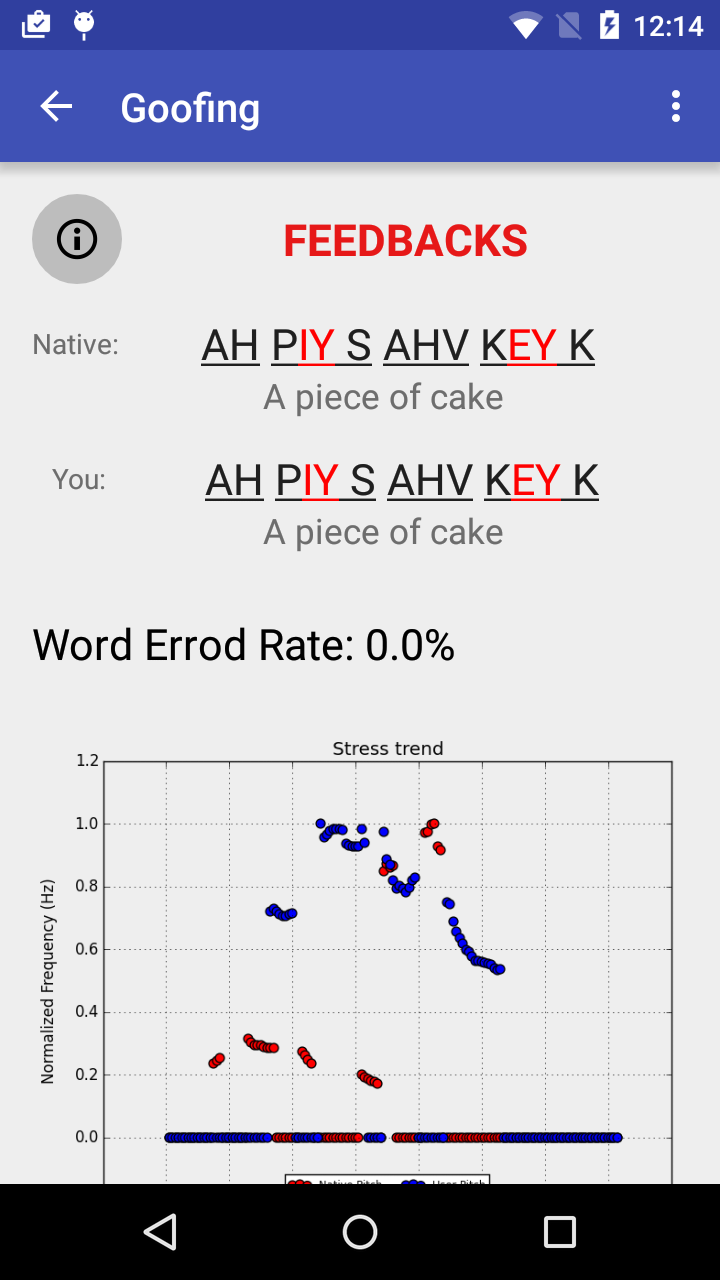
\includegraphics[scale=0.18]{Figures/screenshots/error_rate1.png}
		\caption{Correct pronunciation}
		\label{fig:error_rate_page}
	\end{minipage}%
	\begin{minipage}{.5\textwidth}
		\centering
		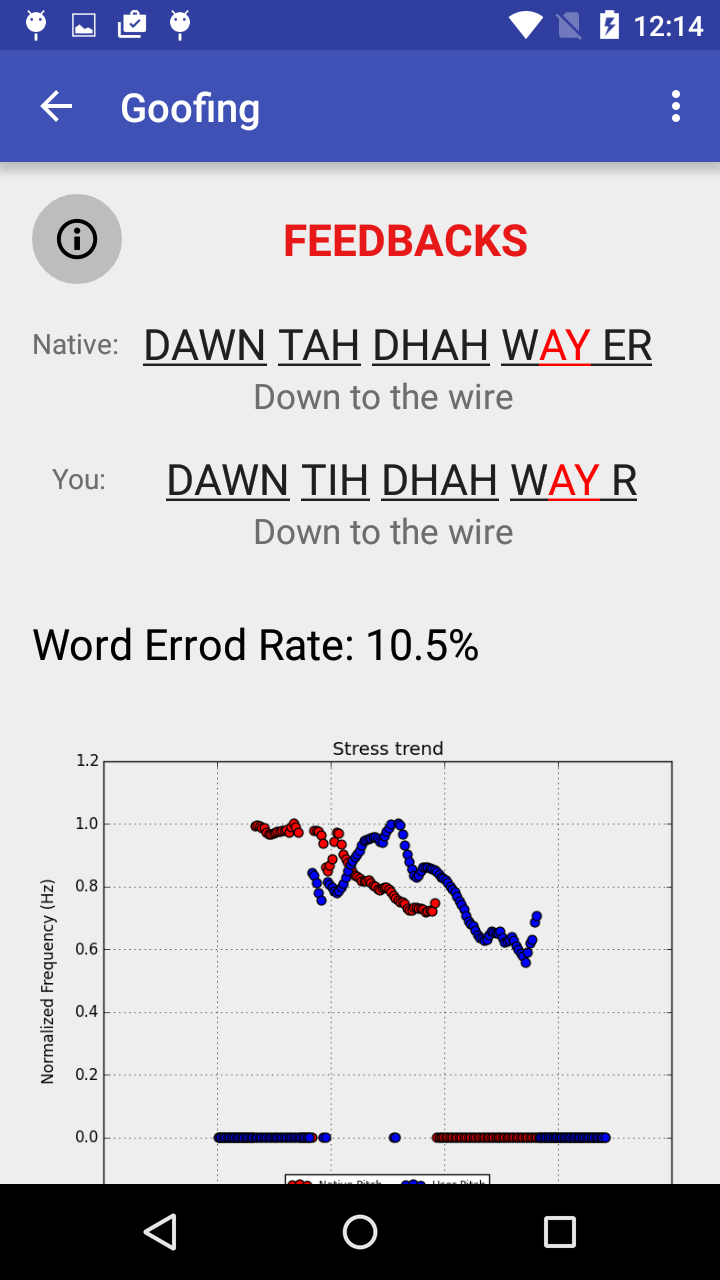
\includegraphics[scale=0.18]{Figures/screenshots/error_rate2.png}
		\caption{Small error in pronunciation}
		\label{fig:error_rate2_page}
	\end{minipage}
\end{figure}

\begin{figure}[!ht]
	\centering
	\begin{minipage}{.5\textwidth}
		\centering
		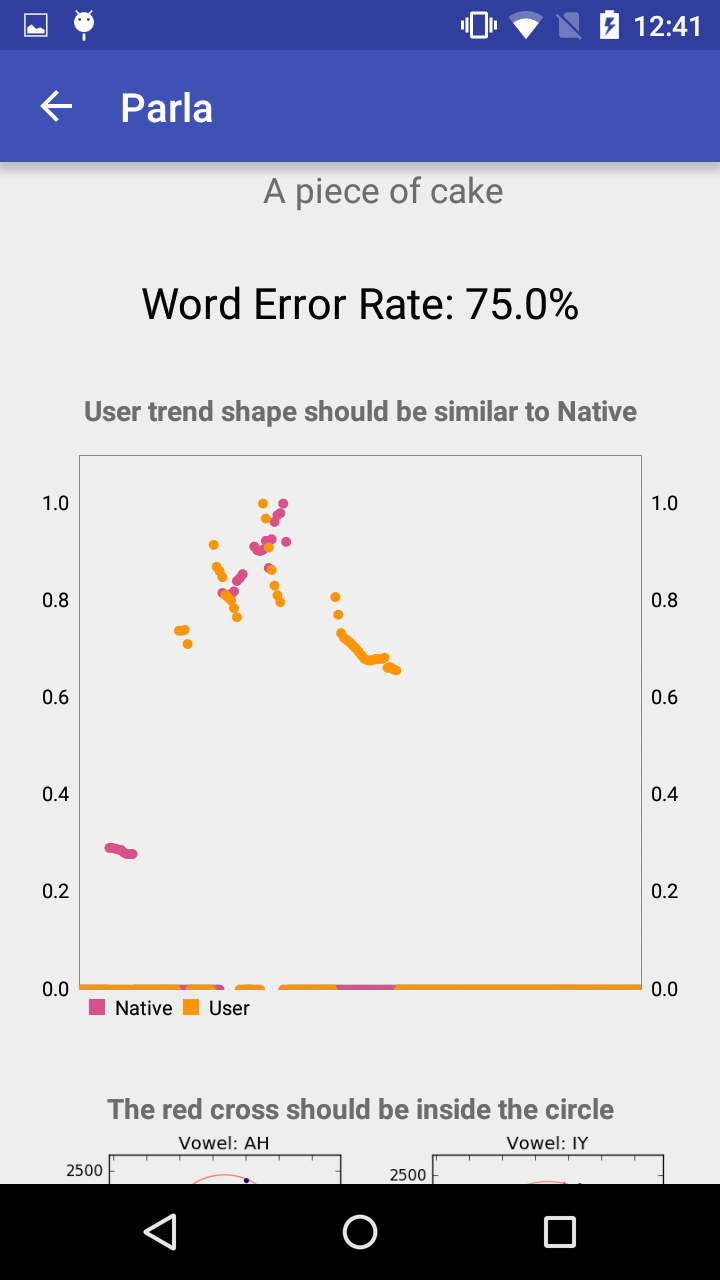
\includegraphics[scale=0.18]{Figures/screenshots/pitch.png}
		\caption{Stress contour chart}
		\label{fig:pitch_page}
	\end{minipage}%
	\begin{minipage}{.5\textwidth}
		\centering
		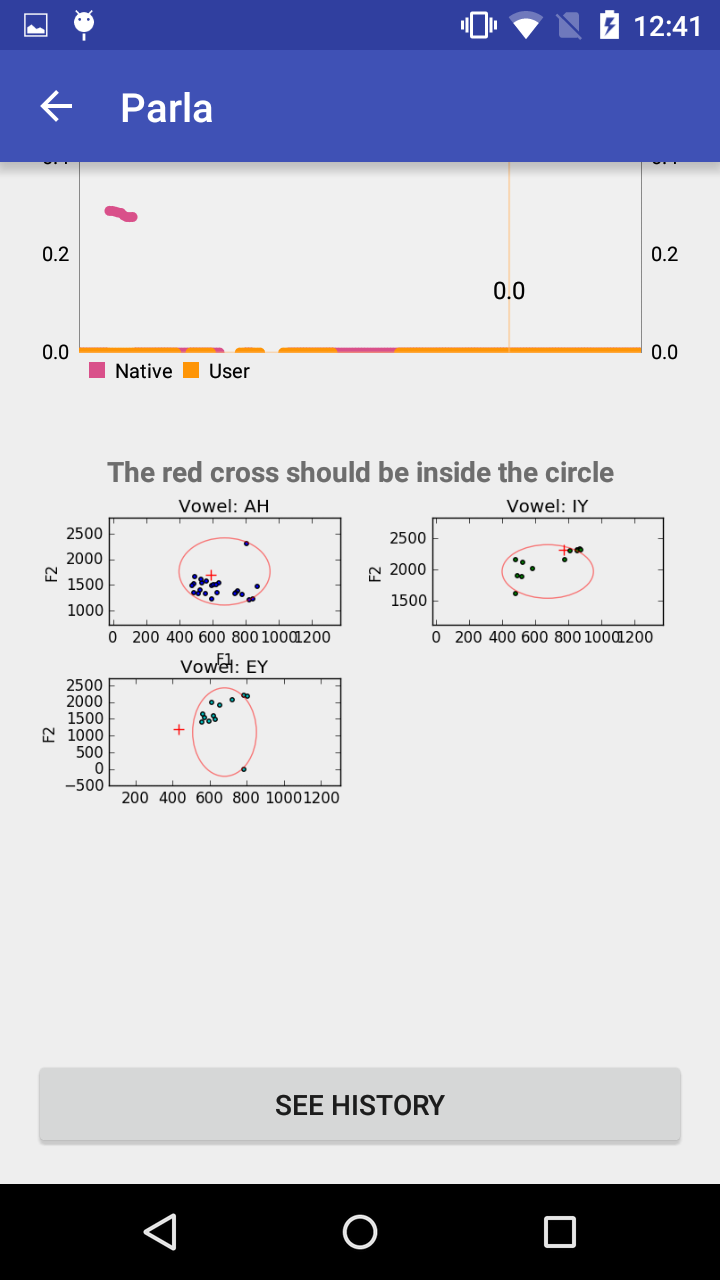
\includegraphics[scale=0.18]{Figures/screenshots/vowels.png}
		\caption{Vowels prediction representation}
		\label{fig:vowels_page}
	\end{minipage}
\end{figure}


\noindent It is important to mention that the user can interact with all the charts. In fact it is possible to zoom in/out and retrieve the value of each single point by tapping on top of the line. This interaction allows users with a linguistic background to have a better numeric-understanding on how the pronunciation was done. \\
\noindent On the very end of this page, the user can navigate directly to the history and see the progress he/she made for that specific sentence.

%%%%% other stuff
